%%%%%%%%%%%%%%%%%%%%%%%%%%%%%%%%%%%%%%%%%%%
%
% From a template maintained at https://github.com/jamesrobertlloyd/cbl-tikz-poster
%
%%%%%%%%%%%%%%%%%%%%%%%%%%%%%%%%%%%%%%%%%%%

\documentclass[portrait,a0b,final,a4resizeable]{a0poster}
\setlength{\paperwidth}{36in} % A0 width: 46.8in
\setlength{\paperheight}{48in} % A0 width: 46.8in

\usepackage{atbegshi}% http://ctan.org/pkg/atbegshi
\AtBeginDocument{\AtBeginShipoutNext{\AtBeginShipoutDiscard}}
\usepackage{qrcode}
\usepackage{multicol}
\usepackage{enumitem}
\usepackage{mathtools}
%\usepackage{color}
%\usepackage{morefloats}
%\usepackage[pdftex]{graphicx}
%\usepackage{rotating}
\usepackage{amsmath, amsthm, amssymb, bm}
%\usepackage{array}
%\usepackage{booktabs}
\usepackage{multirow}
%\usepackage{hyperref}
\usepackage{pgf-soroban}
\usepackage{svg}
\usepackage{bussproofs}
\usepackage{nicematrix}
\usetikzlibrary{cd,shapes.geometric,arrows,chains,matrix,positioning,scopes,calc,trees}
\tikzstyle{mybox} = [draw=white, rectangle]
%\definecolor{darkblue}{rgb}{0,0.08,0.45}
%\definecolor{blue}{rgb}{0,0,1}
%\usepackage{dsfont}
\usepackage[margin=0.5in]{geometry}
%\usepackage{fp}

%%%%%%%%%%%%%%%%%%%%%%%%%%%%%%%%%%%%%%%%%%%
%
% myfig
%
% \myfig - replacement for \figure
% necessary, since in multicol-environment
% \figure won't work
%
%%%%%%%%%%%%%%%%%%%%%%%%%%%%%%%%%%%%%%%%%%%

\newcommand{\myfig}[3][0]{
\begin{center}
    \vspace{1.5cm}
    \includegraphics[width=#3\hsize,angle=#1]{#2}
    \nobreak\medskip
\end{center}}

%%%%%%%%%%%%%%%%%%%%%%%%%%%%%%%%%%%%%%%%%%%
%
% mycaption
%
% \mycaption - replacement for \caption
% necessary, since in multicol-environment \figure and
% therefore \caption won't work
%
%%%%%%%%%%%%%%%%%%%%%%%%%%%%%%%%%%%%%%%%%%%

%\newcounter{figure}
\setcounter{figure}{1}
\newcommand{\mycaption}[1]{
\vspace{0.5cm}
\begin{quote}
{{\sc Figure} \arabic{figure}: #1}
\end{quote}
\vspace{1cm}
\stepcounter{figure}
}

%%%%%%%%%%%%%%%%%%%%%%%%%%%%%%%%%%%%%%%%%%%
%
% Some standard colours
%
%%%%%%%%%%%%%%%%%%%%%%%%%%%%%%%%%%%%%%%%%%%

\definecolor{camlightblue}{rgb}{0.601 , 0.8, 1}
\definecolor{camdarkblue}{rgb}{0, 0.203, 0.402}
\definecolor{camred}{rgb}{1, 0.203, 0}
\definecolor{camyellow}{rgb}{1, 0.8, 0}
\definecolor{lightblue}{rgb}{0, 0, 0.80}
\definecolor{white}{rgb}{1, 1, 1}
\definecolor{whiteblue}{rgb}{0.80, 0.80, 1}

%%%%%%%%%%%%%%%%%%%%%%%%%%%%%%%%%%%%%%%%%%%
%
% Some look and feel definitions
%
%%%%%%%%%%%%%%%%%%%%%%%%%%%%%%%%%%%%%%%%%%%

\setlength{\columnsep}{0.03\textwidth}
\setlength{\columnseprule}{0.0018\textwidth}
\setlength{\parindent}{0.0cm}

%%%%%%%%%%%%%%%%%%%%%%%%%%%%%%%%%%%%%%%%%%%
%
% \mysection - replacement for \section*
%
% Puts a pretty box around some text
% TODO - any other thoughts for what this box should look like
%
%%%%%%%%%%%%%%%%%%%%%%%%%%%%%%%%%%%%%%%%%%%

\tikzstyle{mysection} = [rectangle,
draw=none,
shade,
outer color=camlightblue!30,
inner color=camlightblue!30,
text width=0.965\columnwidth,
text centered,
rounded corners=20pt,
minimum height=0.09\columnwidth]

\newcommand{\mysection}[1]
{
\begin{center}
    \begin{tikzpicture}
        \node[mysection] {\sffamily\bfseries\LARGE#1};
    \end{tikzpicture}
\end{center}
}

%%%%%%%%%%%%%%%%%%%%%%%%%%%%%%%%%%%%%%%%%%%
%
% Set the font
%
% TODO - Not sure what a canonical choice is - feel free to modify
%
%%%%%%%%%%%%%%%%%%%%%%%%%%%%%%%%%%%%%%%%%%%

\renewcommand{\familydefault}{cmss}
\sffamily

%%%%%%%%%%%%%%%%%%%%%%%%%%%%%%%%%%%%%%%%%%%%%%%%%%%%
%%%               Background                     %%%
%%%%%%%%%%%%%%%%%%%%%%%%%%%%%%%%%%%%%%%%%%%%%%%%%%%%

\newcommand{\background}[3]{
%\definecolor{cgradbegin}{#1}
%\definecolor{cgradend}{#2}
% \psframe[fillstyle=gradient,gradend=cgradend,
% gradbegin=cgradbegin,gradmidpoint=#3](0.,0.)(1.\textwidth,-1.\textheight)
}




%%%%%%%%%%%%%%%%%%%%%%%%%%%%%%%%%%%%%%%%%%%%%%%%%%%%
%%%                pcolumn                       %%%
%%%%%%%%%%%%%%%%%%%%%%%%%%%%%%%%%%%%%%%%%%%%%%%%%%%%

\newenvironment{pcolumn}[1]{
\begin{minipage}{#1\textwidth}
\begin{center}
}{
\end{center}
\end{minipage}
}



%%%%%%%%%%%%%%%%%%%%%%%%%%%%%%%%%%%%%%%%%%%%%%%%%%%%
%%%                pbox                          %%%
%%%%%%%%%%%%%%%%%%%%%%%%%%%%%%%%%%%%%%%%%%%%%%%%%%%%

\definecolor{lcolor}{rgb}{0, 0, 0.80}
\definecolor{gcolor1}{rgb}{1, 1, 1}
\definecolor{gcolor2}{rgb}{.80, .80, 1}

% \def\fc{fillcolor}
% \def\getfc #1=#2\par{\def\ffc{#1} \ifx\ffc\fc #2\fi}
% \def\getfillcolor #1,#2\par{\getfc #1\par \getfc #2\par}

%  \newcommand{\psshadowbox}[2]{%[2][magenta]{
%      \fbox{Input arg: #1}
%      \fbox{#1}
%      \fbox {\getfillcolor #1\par}
%      \def\col{\getfillcolor #1\par}

%      \let\coll=\col
%       \coll
%     \colorbox{\col}{#2}
%       \mbox
%   \coloredshadowbox{black}{\coll}{#2}
%   }

\newcommand{\pbox}[4]{
%\psshadowbox[#3]{
%\fbox{
\mbox{
\begin{minipage}[t][#2][t]{#1}
#4
\end{minipage}
}%}
}

%%%%%%%%%%%%%%%%%%%%%%%%%%%%%%%%%%%%%%%%%%%
%
% Poster environment
%
% Centres everything and can be used to define the width of the content
%
%%%%%%%%%%%%%%%%%%%%%%%%%%%%%%%%%%%%%%%%%%%

\newenvironment{poster}{
\begin{center}
\begin{minipage}[c]{\textwidth}
}{
\end{minipage}
\end{center}
}

\def\newarrow{\mbox{\begin{tikzpicture}
\useasboundingbox{(-3pt,-4.5pt) rectangle (19pt,1pt)};
\draw[->] (0,-0.07)--(17pt,-0.07);\end{tikzpicture}}}

%%%%%%%%%%%%%%%%%%%%%%%%%%%%%%%%%%%%%%%%%%%
%
% Bottom box
%
%%%%%%%%%%%%%%%%%%%%%%%%%%%%%%%%%%%%%%%%%%%

\newlength{\bottomboxheight}
\setlength{\bottomboxheight}{0.1\paperheight}

\newcommand{\bottombox}[1]{\vfill
\noindent\colorbox{white}{
\begin{minipage}[c][\bottomboxheight][c]{\textwidth}
\centering
\begin{minipage}{0.9\textwidth}
\vfill{

\fontsizesection\color{black}
#1
}

\end{minipage}
\end{minipage}

}
}

%% Bottom box logo
\newcommand{\bottomboxlogo}[2][width=\textwidth]{
\begin{minipage}[c][\bottomboxheight][c]{0.3\textwidth}
\raggedleft\includegraphics[#1]{#2}
\end{minipage}
}

\newcommand{\bottomboxlogoleft}[2][width=\textwidth]{
\begin{minipage}[l][\bottomboxheight][c]{0.3\textwidth}
\raggedleft\includegraphics[#1]{#2}
\end{minipage}
}

%%%%%%%%%%%%%%%%%%%%%%%%%%%%%%%%%%%%%%%%%%%
%
% Highlighting
%
%%%%%%%%%%%%%%%%%%%%%%%%%%%%%%%%%%%%%%%%%%%

\definecolor{slightgray}{rgb}{0.90, 0.90, 0.90}

\usepackage{soul}
\makeatletter
\def\SOUL@hlpreamble{%
\setul{}{3.0ex}%
\let\SOUL@stcolor\SOUL@hlcolor%
\SOUL@stpreamble%
}
\makeatother

\newcommand{\inline}[1]{%
\begingroup%
\sethlcolor{slightgray}%
\hl{\ttfamily\small #1}%
\endgroup
}

\newcommand{\tinline}[1]{%
\begingroup%
\sethlcolor{slightgray}%
\hl{\ttfamily #1}%
\endgroup
}

%%%%%%%%%%%%%%%%%%%%%%%%%%%%%%%%%%%%%%%%%%%
%
% Kotlin syntax highlighting
%
%%%%%%%%%%%%%%%%%%%%%%%%%%%%%%%%%%%%%%%%%%%

\usepackage[skins,breakable,listings]{tcolorbox}

\usepackage[dvipsnames]{xcolor}
\usepackage[table]{xcolor}
\lstdefinelanguage{kotlin}{
comment=[l]{//},
commentstyle={\color{gray}\ttfamily},
emph={delegate, filter, firstOrNull, forEach, it, lazy, mapNotNull, println, @Repeat, return@},
emphstyle={\color{OrangeRed}},
identifierstyle=\color{black},
keywords={abstract, actual, as, as?, break, by, class, companion, continue, data, do, dynamic, else, enum, expect, false, final, for, fun, get, if, import, in, infix, interface, internal, is, null, object, open, operator, override, package, private, public, return, sealed, set, super, suspend, this, throw, true, try, typealias, val, var, vararg, when, where, while, tailrec, reified},
keywordstyle={\color{blue}\bfseries},
morecomment=[s]{/*}{*/},
morestring=[b]",
morestring=[s]{"""*}{*"""},
ndkeywords={@Deprecated, @JvmField, @JvmName, @JvmOverloads, @JvmStatic, @JvmSynthetic, Array, Byte, Double, Float, Int, Integer, Iterable, Long, Runnable, Short, String},
ndkeywordstyle={\color{BurntOrange}\bfseries},
sensitive=true,
stringstyle={\color{ForestGreen}\ttfamily},
literate={`}{{\char0}}1
}

%%%%%%%%%%%%%%%%%%%%%%%%%%%%%%%%%%%%%%%%%%%
%
% Color boxes
%
%%%%%%%%%%%%%%%%%%%%%%%%%%%%%%%%%%%%%%%%%%%

\tcbset{
enhanced jigsaw,
breakable,
listing only,
boxsep=-1pt,
top=-1pt,
bottom=-0.5pt,
right=-0.5pt,
overlay first={
\node[black!50] (S) at (frame.south) {\Large\ding{34}};
\draw[dashed,black!50] (frame.south west) -- (S) -- (frame.south east);
},
overlay middle={
\node[black!50] (S) at (frame.south) {\Large\ding{34}};
\draw[dashed,black!50] (frame.south west) -- (S) -- (frame.south east);
\node[black!50] (S) at (frame.north) {\Large\ding{34}};
\draw[dashed,black!50] (frame.north west) -- (S) -- (frame.north east);
},
overlay last={
\node[black!50] (S) at (frame.north) {\Large\ding{34}};
\draw[dashed,black!50] (frame.north west) -- (S) -- (frame.north east);
},
before={\par\vspace{10pt}},
after={\par\vspace{\parskip}\noindent}
}

\newtcblisting{kotlinlisting}[1][]{%
width=20.5cm,
left=20pt,
top=5pt,
listing options={
language=kotlin,
basicstyle=\ttfamily\normalsize,
%numberstyle=\footnotesize,
showstringspaces=false,
tabsize=2,
breaklines=true,
numbers=none,
inputencoding=utf8,
escapeinside={(*}{*)},
#1
},
underlay unbroken and first={%
\path[draw=none] (interior.north west) rectangle node[white]{
\includegraphics[width=10mm]{../figures/kotlin_file.png}} ([xshift=-18mm,yshift=-20mm]interior.north west);
}
}

\newtcblisting{pythonlisting}[1][]{
width=17cm,
left=20pt,
top=5pt,
listing options={
language=Python,
basicstyle=\ttfamily\normalsize,
upquote=true,
breaklines=true,
showstringspaces=false,
keywordstyle=\color{blue}\bfseries,
escapeinside={(*}{*)},
#1
},
fonttitle=\ttfamily\small,
underlay unbroken and first={
\path[draw=none] (interior.north west) rectangle node[white]{\includegraphics[width=10mm]{../figures/python_icon.png}} ([xshift=-18mm,yshift=-20mm]interior.north west);
}
}

% Imitate syntax error
\usepackage{ulem}
\makeatletter
\def\uwave{\bgroup \markoverwith{\lower7.5\p@\hbox{\sixly \textcolor{red}{\char58}}}\ULon}
\font\sixly=lasy6 % does not re-load if already loaded, so no memory problem.
\makeatother

\usepackage{tikz}
\usepackage[skins,breakable,listings]{tcolorbox}
\usepackage{pgfplots}
\usepackage{tikz-qtree}
\usepackage{graphicx}

\usepackage{include/preamble}


% Custom notation
\newcommand{\fdeep}{\vf^{(1:L)}}
\newcommand{\flast}{\vf^{(L)}}
\newcommand{\Jx}{J_{\vx \rightarrow \vy}}
\newcommand{\Jxx}{J_{\vx \rightarrow \vy}(\vx)}
\newcommand{\Jy}{J_{\vy \rightarrow \vx}}
\newcommand{\Jyy}{J_{\vy \rightarrow \vx}(\vy)}
\newcommand{\detJyy}{ \left| J_{\vy \rightarrow \vx}(\vy) \right|}

\newcommand\transpose{{\textrm{\tiny{\sf{T}}}}}
\newcommand{\note}[1]{}
\newcommand{\hlinespace}{~\vspace*{-0.15cm}~\\\hline\\\vspace*{0.15cm}}
\newcommand{\embeddingletter}{g}
\newcommand{\bo}{{\sc bo}}
\newcommand{\agp}{Arc \gp}

\newcommand{\D}{\mathcal{D}}
\newcommand{\X}{\mathbf{X}}
\newcommand{\y}{y}
\newcommand{\data} {\X, \y}
\newcommand{\x}{\mathbf{x}}
\newcommand{\f}{\mathit{f}}

\newcommand{\fx}{ f(\mathbf{x}) }
\newcommand{\U}{\mathcal{U}}
\newcommand{\E}{\mathbf{E}}


\newcommand{\bardist}[0]{\hspace{-0.2cm}}

\newlength{\arrowsize}
\pgfarrowsdeclare{biggertip}{biggertip}{
\setlength{\arrowsize}{10pt}
\addtolength{\arrowsize}{2\pgflinewidth}
\pgfarrowsrightextend{0}
\pgfarrowsleftextend{-5\arrowsize}
}{
\setlength{\arrowsize}{1pt}
\addtolength{\arrowsize}{\pgflinewidth}
\pgfpathmoveto{\pgfpoint{-5\arrowsize}{4\arrowsize}}
\pgfpathlineto{\pgfpointorigin}
\pgfpathlineto{\pgfpoint{-5\arrowsize}{-4\arrowsize}}
\pgfusepathqstroke
}


% Custom commmands.

\def\jointspacing{\vspace{0.3in}}

\def\boxwidth{0.21\columnwidth}
\newcommand{\gpdrawbox}[1]{
\setlength\fboxsep{0pt}
\hspace{-0.36in}
\fbox{\hspace{-4mm}
%\includegraphics[width=\boxwidth]{../figures/deep_draws/deep_gp_sample_layer_#1}
\hspace{-4mm}}}

\newcommand{\mappic}[1]{
%\hspace{-0.05in}\includegraphics[width=\boxwidth]{../../figures/seed-0-map/latent_coord_map_layer_#1}
}

\newcommand{\mappiccon}[1]{
%\hspace{-0.05in}\includegraphics[width=\boxwidth]{../../figures/seed-0-map-connected/latent_coord_map_layer_#1}
}

\newcommand{\spectrumpic}[1]{
%\includegraphics[trim=4.5mm 0mm 4mm 3mm, clip, width=0.44\columnwidth]{../figures/spectrum/layer-#1}
}

\usepackage{dsfont}

\newcommand{\feat}{\vh}
\newcommand{\bs}{\blacksquare}
\newcommand{\ws}{\square}

\tikzset{
  treenode/.style = {shape=rectangle, rounded corners,
  draw, align=center,
  top color=white, bottom color=blue!20},
  root/.style     = {treenode, font=\tiny, bottom color=red!30},
  env/.style      = {treenode, font=\tiny},
  dummy/.style    = {circle,draw}
}


\begin{document}
  \begin{poster}
    \vspace{-0.3cm}
    %%% Header
    \begin{center}
      \begin{pcolumn}{1.03}
        %%% Title
        \begin{minipage}[c][9cm][c]{0.85\textwidth}
          \begin{center}
          {\Huge \textbf{Let's wrap this up! Incremental structured decoding with resource constraints}}\\[10mm]
          {\huge Breandan Considine}
          \end{center}
        \end{minipage}
      \end{pcolumn}
    \end{center}

    \vspace*{-0.5cm}

    \large


    %%%%%%%%%%%%%%%%%%%%%%%%%%%%%%%%%%%%%%%%%%%%%%%%%%%%%%%%%%%%%%%%%%%%%%
    %%% Beginning of Document
    %%%%%%%%%%%%%%%%%%%%%%%%%%%%%%%%%%%%%%%%%%%%%%%%%%%%%%%%%%%%%%%%%%%%%%

    \Large

    \begin{multicols}{2}


      \mysection{Main Idea}

      \vspace*{-1cm}
      \null\hspace*{2.5cm}\begin{minipage}[c]{0.88\columnwidth}
      \renewcommand\labelitemi{$\vcenter{\hbox{\small$\bullet$}}$}
      \begin{itemize}
%        \item Sampling with rejection is unnecessary if you can map onto a simpler distribution
        \item \phantom{\small{.}} Language models have trouble with single-shot constraint satisfaction
        \item \phantom{\small{.}} Typically solved via rejection sampling or backtracking style decoders
        \item \phantom{\small{.}} We implement an incremental structured decoder for autoregressive LLMs
        \item \phantom{\small{.}} Guarantees monotonic progress and preservation of resource constraints
        \item \phantom{\small{.}} Ensures all valid words are generable and all generable words are valid
      \end{itemize}
      \end{minipage}

\jointspacing

\mysection{Motivation}
\null\hspace*{3cm}\begin{minipage}[c]{0.85\columnwidth}
Suppose we want to force an autoregressive LLM to generate syntactically valid next tokens $P(x_n \mid x_1, \ldots, x_{n-1})$, under certain resource constraints. Here is a concrete example: ``Generate an arithmetic expression with two or more variables in ten or fewer tokens.''. If we sample the partial trajectory,
\begin{center}\texttt{( x + ( y * }\underline{\texttt{(}}\end{center}\\
then we will spend quite a long time rejecting invalid completions, because this trajectory has past the point of no return. Even though \texttt{(} is a locally valid continuation, we need to avoid this scenario, because we would like a linear sampling delay and to guarantee this, we must avoid backtracking.
\end{minipage}

      \jointspacing

      \mysection{Semiring Parsing}
      \null\hspace*{3cm}\begin{minipage}[c]{0.85\columnwidth}
          Given a CFG, $G: \mathcal{G} = \langle V, \Sigma, P, S\rangle$, in Chomsky Normal Form (CNF), we may construct a recognizer $R_\mathcal{G}: \Sigma^n \rightarrow \mathbb{B}$ for strings $\sigma: \Sigma^n$ as follows. Let $2^V$ be our domain, where $0$ is $\varnothing$, $\oplus$ is $\cup$, and $\otimes$ be defined as:\vspace{1cm}
      \end{minipage}

      \[
        s_1 \otimes s_2 = \{C \mid \langle A, B\rangle \in s_1 \times s_2, (C\rightarrow AB) \in P\}
      \]

      \null\hspace*{3cm}\begin{minipage}[c]{0.85\columnwidth}
If we define $\hat\sigma_r = \{w \mid (w \rightarrow \sigma_r) \in P\}$, then construct a matrix with unit nonterminals on the superdiagonal, $M_0[r+1=c](G, \sigma) = \;\hat\sigma_r$ the fixpoint $M_{i+1} = M_i + M_i^2$ is fully determined by the first diagonal:\vspace{0.5cm}
\end{minipage}

\begin{align*}
\hspace{-0.5cm}\resizebox{.86\columnwidth}{!}{
$M$_0 =
\begin{pNiceMatrix}[xdots/line-style=loosely dotted]
   \varnothing & \hat\sigma_1 & \varnothing & \Cdots & \varnothing \\
   \Vdots      & \Ddots       & \Ddots      & \Ddots & \Vdots\\
               &              &             &        & \varnothing\\
               &              &             &        & \hat\sigma_n \\
   \varnothing & \Cdots       &             &        & \varnothing
\end{pNiceMatrix} \Rightarrow
\begin{pNiceMatrix}[xdots/line-style=loosely dotted]
  \varnothing & \hat\sigma_1 & \Lambda & \Cdots & \varnothing \\
  \Vdots      & \Ddots       & \Ddots  & \Ddots & \Vdots\\
              &              &         &        & \Lambda\\
              &              &         &        & \hat\sigma_n \\
  \varnothing & \Cdots       &         &        & \varnothing
\end{pNiceMatrix} \Rightarrow \ldots \Rightarrow M_\infty =
\begin{pNiceMatrix}[xdots/line-style=loosely dotted]
   \varnothing & \hat\sigma_1 & \Lambda & \Cdots & \Lambda^*_\sigma\\
   \Vdots      & \Ddots       & \Ddots  & \Ddots & \Vdots\\
               &              &         &        & \Lambda\\
               &              &         &        & \hat\sigma_n \\
   \varnothing & \Cdots       &         &        & \varnothing
\end{pNiceMatrix}
}
\end{align*}

\null\hspace*{3cm}\begin{minipage}[c]{0.85\columnwidth}
CFL membership is recognized by $R(G, \sigma) = [S \in \Lambda^*_\sigma] \Leftrightarrow [\sigma \in \mathcal{L}(G)]$.
\end{minipage}

      \jointspacing

      \mysection{Porous Completion}

      \null\hspace*{3cm}\begin{minipage}[c]{0.85\columnwidth}
      Let us consider an example with two holes, $\sigma = 1$ \underline{\hspace{1cm}} \underline{\hspace{1cm}}, with the grammar being $G=\{S\rightarrow N O N, O \rightarrow + \mid \times, N \rightarrow 0 \mid 1\}$. This can be rewritten into CNF as $G'=\{S \rightarrow N L, N \rightarrow 0 \mid 1, O \rightarrow \times \mid +, L \rightarrow O N\}$.\vspace{0.5cm}
      \end{minipage}

      \null\hspace*{2.7cm}\begin{minipage}[c]{\columnwidth}
                      \resizebox{.85\columnwidth}{!}{
                      {\renewcommand{\arraystretch}{1.2}
\begin{tabular}{|c|c|c|c|}
  \hline
  & $2^V$ & $\mathbb{B}^{|V|}$ & $\mathbb{B}^{|V|}\rightarrow\mathbb{B}^{|V|}$\\\hline
  $M_0$ & \begin{pmatrix}
  \phantom{V} & \tiny{\{N\}} &         &             \\
              &              & \{N,O\} &             \\
              &              &         & \{N,O\} \\
              &              &         &
  \end{pmatrix} & \begin{pmatrix}
  \phantom{V} & \ws\bs\ws\ws &              &              \\
              &              & \ws\bs\bs\ws &              \\
              &              &              & \ws\bs\bs\ws \\
              &              &              &
  \end{pmatrix} & \begin{pmatrix}
     \phantom{V} & V_{0, 1} &          &          \\
                 &          & V_{1, 2} &          \\
                 &          &          & V_{2, 3} \\
                 &          &          &
  \end{pmatrix} \\\hline
  $M_1$ & \begin{pmatrix}
  \phantom{V} & \tiny{\{N\}} & \varnothing &         \\
              &              & \{N,O\}     & \{L\}   \\
              &              &             & \{N,O\} \\
              &              &             &
  \end{pmatrix} & \begin{pmatrix}
  \phantom{V} & \ws\bs\ws\ws & \ws\ws\ws\ws &              \\
              &              & \ws\bs\bs\ws & \bs\ws\ws\ws \\
              &              &              & \ws\bs\bs\ws \\
              &              &              &
  \end{pmatrix} & \begin{pmatrix}
  \phantom{V} & V_{0, 1} & V_{0, 2} &          \\
              &          & V_{1, 2} & V_{1, 3} \\
              &          &          & V_{2, 3} \\
              &          &          &
  \end{pmatrix} \\\hline
  $M_\infty$ & \begin{pmatrix}
  \phantom{V} & \tiny{\{N\}} & \varnothing & \{S\}   \\
              &              & \{N,O\}     & \{L\}   \\
              &              &             & \{N,O\} \\
              &              &             &
  \end{pmatrix} & \begin{pmatrix}
  \phantom{V} & \ws\bs\ws\ws & \ws\ws\ws\ws & \ws\ws\ws\bs \\
              &              & \ws\bs\bs\ws & \bs\ws\ws\ws \\
              &              &              & \ws\bs\bs\ws \\
              &              &              &
  \end{pmatrix} & \begin{pmatrix}
  \phantom{V} & V_{0, 1} & V_{0, 2} & V_{0, 3} \\
              &          & V_{1, 2} & V_{1, 3} \\
              &          &          & V_{2, 3} \\
              &          &          &
  \end{pmatrix}\\\hline
\end{tabular}\\
}
                      }\vspace{0.4cm}
      \end{minipage}

      \null\hspace*{3cm}\begin{minipage}[c]{0.90\columnwidth}
      This procedure decides if $\exists \sigma' \in \mathcal{L}(G) \mid \sigma' \sqsubseteq \sigma$ but forgets provenance.
\vspace{1cm}
      \end{minipage}
      \jointspacing

\pagebreak
      \mysection{Regular Expression Propagation}
      \jointspacing

      \hspace*{2cm}\begin{minipage}[c]{0.90\columnwidth}
Regular expressions that permit union, intersection and concatenation are called generalized regular expressions (GREs). These can be constructed as follows:
\end{minipage}

\vspace{-2cm}
\setlength{\columnseprule}{0pt}
\setlength{\columnsep}{-3cm}
\begin{multicols}{2}
\begin{eqnarray*}
\mathcal{L}(& \varnothing & ) = \varnothing \\
\mathcal{L}(& \varepsilon & ) = \{\varepsilon\} \\
\mathcal{L}(& a           & ) = \{a\}\\
\mathcal{L}(& R\cdot S    & ) = \mathcal{L}(R) \times \mathcal{L}(S)
\end{eqnarray*} \break\vspace{-0.45cm}
\begin{eqnarray*}
\mathcal{L}(& R^*         & ) = \{\varepsilon\} \cup \mathcal{L}(R\cdot R^*)\\
\mathcal{L}(& R\vee S     & ) = \mathcal{L}(R) \cup \mathcal{L}(S)\\
\mathcal{L}(& R\land S    & ) = \mathcal{L}(R) \cap \mathcal{L}(S)\\
\mathcal{L}(& \neg R      & ) = \Sigma^* \setminus \mathcal{L}(R)
\end{eqnarray*}
\end{multicols}

\jointspacing

\hspace*{2cm}\begin{minipage}[c]{0.90\columnwidth}
Finite slices of a CFL are finite and therefore regular a fortiori. Just like sets, bitvectors and other datatypes, we can also propagate GREs through a parse chart. Here, the algebra will carry $\text{GRE}^{|V|}$, where 0 is $\varnothing$, and $\oplus, \otimes$ are defined:
\end{minipage}

\vspace{-2cm}
\setlength{\columnseprule}{0pt}
\setlength{\columnsep}{-2cm}
\begin{multicols}{2}
\begin{eqnarray*}
\hspace{3cm}s_1\otimes s_2 = \Big[\bigvee_{(v \rightarrow AB) \in P} s_1[A] \cdot s_2[B] \Big]_{v \in V} \\
\end{eqnarray*} \break\vspace{-0.45cm}
\begin{eqnarray*}
\phantom{--}s_1\oplus s_2 = \big[s_1[v] \vee s_2[v]\big]_{v \in V} \\
\end{eqnarray*}
\end{multicols}

\hspace*{2cm}\begin{minipage}[c]{0.90\columnwidth}
Initially, we have $M_0[r+1=c](G, \sigma) = \Sigma$.
Now after computing the fixpoint, when we unpack $\Lambda^*_\sigma[S]$, this will be a GRE recognizing the finite CFL slice.
\end{minipage}

\jointspacing

      \mysection{Brzozowski Differentiation}

      \jointspacing

      \hspace*{2cm}\begin{minipage}[c]{0.90\columnwidth}
Janusz Brzozowski (1964) introduced a derivative operator $\partial_a: \textsc{Reg} \rightarrow \textsc{Reg}$, which slices a given prefix off a language: $\partial_a L = \{b \in \Sigma^* \mid ab \in L\}$. The Brzozowski derivative over a GRE is effectively a normalizing rewrite system:
      \end{minipage}

\vspace{-1cm}
\begin{multicols}{2}
\begin{eqnarray*}
\phantom{--}\partial_a & \varnothing & = \varnothing                                           \\
\phantom{--}\partial_a & \varepsilon & = \varnothing                                           \\
\phantom{--}\partial_a & a           & = \varepsilon                                           \\
\phantom{--}\partial_a & b           & = \varnothing  \text{ for each } a \neq b               \\
\phantom{--}\partial_a & R^*         & = (\partial_x R)\cdot R^*                               \\
\phantom{--}\partial_a & \neg R      & = \neg \partial_a R                                     \\
\phantom{--}\partial_a & R\cdot S    & = (\partial_a R)\cdot S \vee \delta(R)\cdot\partial_a S \\
\phantom{--}\partial_a & R\vee S     & = \partial_a R \vee \partial_a S                        \\
\phantom{--}\partial_a & R\land S    & = \partial_a R \land \partial_a S
\end{eqnarray*} \break\vspace{-0.45cm}
\begin{eqnarray*}
\delta(& \varnothing &)= \varnothing                                      \\
\delta(& \varepsilon &)= \varepsilon                                      \\
\delta(& a           &)= \varnothing                                      \\
\delta(& R^*         &)= \varepsilon                                      \\
\delta(& \neg R      &)= \varepsilon \text{ if } \delta(R) = \varnothing  \\
\delta(& \neg R      &)= \varnothing \text{ if } \delta(R) = \varepsilon  \\
\delta(& R\cdot S    &)= \delta(R) \land \delta(S)                        \\
\delta(& R\vee S     &)= \delta(R) \vee  \delta(S)                        \\
\delta(& R\land S    &)= \delta(R) \land \delta(S)
\end{eqnarray*}
\end{multicols}

    \hspace*{2cm}\begin{minipage}[c]{0.90\columnwidth}
    The key property we care about is, this formulation allows us to sample lazily from language intersections, without first materializing the product automaton.
    \end{minipage}

    \jointspacing

      \mysection{Example: Determinantal Point Processes}

      \jointspacing

      \hspace*{2cm}\begin{minipage}[c]{0.90\columnwidth}
      Consider a time series, $A$, whose points which are not too close nor far apart, and $n \leq \sum_{i=1}^{|A|} \mathbf{1}[A_i = \bs]$. We want to sample the typical set using an LLM.\vspace{0.5cm}
\begin{itemize}[leftmargin=2cm]
\item The words are bitvectors of some length, $T$, i.e., $A = \{\ws, \bs\}^T$
\item Consecutive $\bs$ separated by $\ws^{[a,b]}$, i.e., $B = \ws^*(\bs\ws^{[a, b]})^{[n,\infty)}\{\bs,\epsilon\}\ws^*$
\end{itemize}\vspace{0.5cm}

The DPP language is regular. Let $C$ be an FSA such that $\mathcal{L}(C) = \mathcal{L}(A) \cap \mathcal{L}(B)$. For example, here is the minimal automaton for $T=13, a=3, b=5, n=2$.
      \end{minipage}

\jointspacing

\hspace{5cm}\resizebox{0.7\columnwidth}{!}{
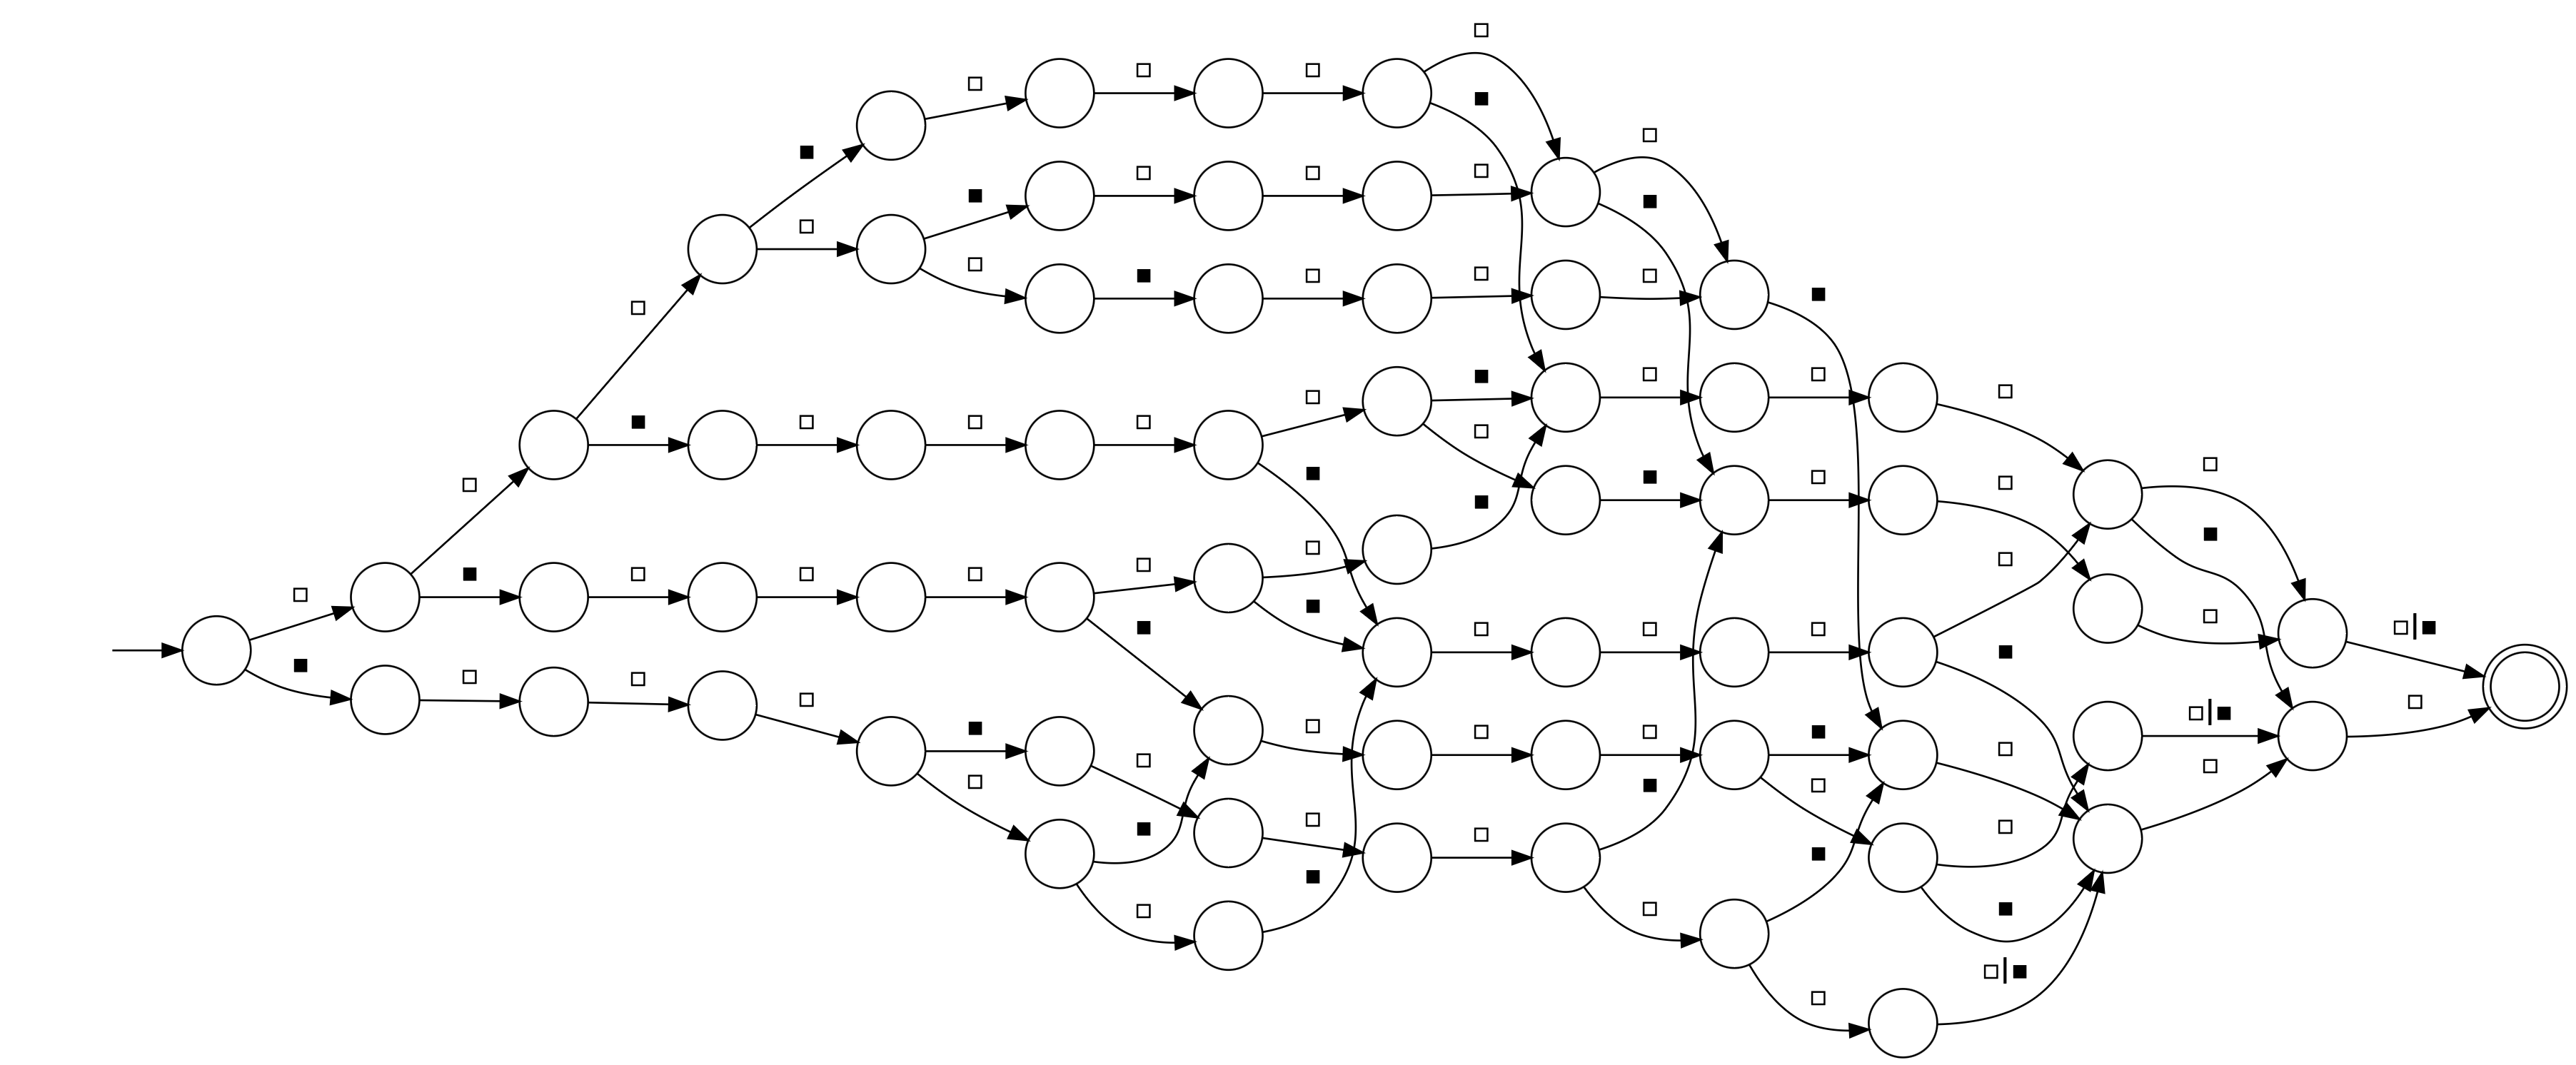
\includegraphics{dpp.png}
%\includesvg{rpp.svg}
}

\jointspacing

      \hspace*{2cm}\begin{minipage}[c]{0.90\columnwidth}
This automaton for $\mathcal{L}(C)$ can grow very large, and we may only need to sample a small sublanguage with distributional support.
Question: Can we incrementally subsample $\mathcal{L}(C)$ while ensuring partial trajectories always lead to acceptance?
\vspace{2cm}
      \end{minipage}

      \jointspacing

    \end{multicols}

    \vspace{-2.2cm}
    \bottombox{
    %% QR code
    %    \hfill\bottomboxlogo{img/kotlin_logo.png}
    % Comment out the line below out to hide logo

    \hspace{1.8cm}
    \begin{minipage}[c][0.1\paperheight][c]{0.18\textwidth}\qrcode[height=2.6in]{https://tidyparse.github.io/} \end{minipage}
    \begin{minipage}[c][0.1\paperheight][c]{0.25\textwidth}
\includegraphics[height=2.6in]{../figures/tidyparse_logo.png} \end{minipage}
    \hspace{-4cm}
    \begin{minipage}[c][0.1\paperheight][c]{0.33\textwidth}
\includegraphics[height=3in]{../figures/mcgill.png} \end{minipage}
    \hspace{2cm}
    \begin{minipage}[c][0.1\paperheight][c]{0.33\textwidth}
\includegraphics[height=3.2in]{../figures/mila.png} \end{minipage}
    %    \hfill\bottomboxlogo{img/mila_mauve.png} % \hfill shifts the logo across so it meets the right hand side margin
    % Note that \bottomboxlogo takes an optional width argument. It defaults to the following:
    % \hfill\bottomboxlogo[width=\textwidth]{<path_to_image_file>}
    % where \textwidth is actually the width of a minipage which is defined in the \bottombox command of
    % betterportaitposter.cls It's a standard \includegraphics command in there, so easy to change if
    % you need to add a border etc.
    }
\end{poster}
\end{document}
